\documentclass[a4paper]{article}

\usepackage[portuguese]{babel}
\usepackage[utf8]{inputenc}
\usepackage{indentfirst}
\usepackage{graphicx}
\usepackage{verbatim}
\usepackage{float}
\usepackage{listings}
\usepackage{float}
\usepackage{listings}
\usepackage{url}
\usepackage{color}
\usepackage{minted}
\usepackage{mdframed}

\lstset{emph={%  
   {:-}%
     },emphstyle={\color{red}\bfseries\underbar}%
}%

\definecolor{mintedbackground}{rgb}{0.95,0.95,0.95}


\begin{document}

\setlength{\textwidth}{16cm}
\setlength{\textheight}{22cm}

\title{\Huge\textbf{\textit{Crab Stack}}\linebreak\linebreak\linebreak
\Large\textbf{Relatório Final}\linebreak\linebreak
\linebreak\linebreak

\includegraphics[scale=0.1]{img/feup-logo.png}\linebreak\linebreak
\linebreak\linebreak
\Large{Mestrado Integrado em Engenharia Informática e Computação} \linebreak\linebreak
\Large{Programação em Lógica}\linebreak
}

\author{\textbf{Grupo Crab\textunderscore Stack\textunderscore 1:}\\
Inês de Sousa Caldas - up200904082 \\
Maria Teresa Chaves - up201306842 \\
\linebreak\linebreak \\
 \\ Faculdade de Engenharia da Universidade do Porto \\ Rua Roberto Frias, s\/n, 4200-465 Porto, Portugal \linebreak\linebreak\linebreak
\linebreak\linebreak\vspace{1cm}}

\maketitle
\thispagestyle{empty}

%************************************************************************************************
%************************************************************************************************

\newpage

\section*{Resumo}
No âmbito da unidade curricular de  Programação em Lógica  foi desenvolvido o jogo \textit{Crab Stack} em ambiente de \textit{Sicstus Prolog}. Neste jogo, cada jogador tem um conjunto de caranguejos que pode mover no tabuleiro de acordo com um conjunto de regras. O objetivo é fazer com que o adversário fique sem jogadas possíveis. \\

Para implementar o jogo dividiu-se o jogo nas suas diversas fases. O desenvolvimento da aplicação consistiu na representação de um tabuleiro hexagonal, composto por células que representam rochas, onde os caranguejos estão posicionados, podendo estes apenas mover-se para cima de rochas habitadas por outros caranguejos. Implementou-se inicialmente um menu de forma a que fosse intuitivo para o utilizador jogar o \textit{Crab Stack} em modo texto. Depois partiu-se para a implementação da mecânica do jogo, começando pelo início do jogo em que as peças são distribuídas pelo tabuleiro de forma aleatória. Posteriormente, implementou-se o movimento de uma peça no tabuleiro, verificando sempre se após o movimento, este provocava uma onda (descrita nas regras de jogo). Por último, foi implementado o final do jogo para verificar se um dos jogadores teria ganho.\\

Assim, o resultado do presente trabalho é uma aplicação que representa e implementa o jogo \textit{Crab Stack} e que mostra ao utilizador uma interface em modo texto intuitiva. O jogo permite também escolher o modo de jogo que inclui  Humano vs Humano, Humano vs Máquina ou mesmo Máquina vs Máquina.\\

\newpage

\tableofcontents

\newpage
%%%%%%%%%%%%%%%%%%%%%%%%%%
\section{Introdução}

Este trabalho teve como objetivo a implementação, em linguagem Prolog, de um jogo de tabuleiro para dois jogadores. Um jogo de tabuleiro caracteriza-se pelo tipo de tabuleiro e de peças, pelas regras de movimentação das peças (jogadas possíveis) e pelas condições de terminação do jogo com derrota, vitória ou empate. Também teve como objetivo a implementação da aplicação de forma a que fosse possível jogar em três modos de utilização: Humano vs Humano, Humano vs Computador e Computador vs Computador. No caso de algum dos modos escolhidos incluir o computador, é possível escolher qual o nível de dificuldade do mesmo. Por último, teve também como objetivo a implementação de uma interface adequada com o utilizador, em modo de texto.~\cite{enunciado_trabalho}\\

Este trabalho, teve como motivação uma aprendizagem didática da linguagem Prolog e um aprofundamento e maturação dos conhecimentos transmitidos na unidade curricular de Programação em Lógica.
Outra grande motivação, foi a aprendizagem de conceitos de inteligência artificial em ambiente de jogo, como os algoritmos de \textit{minimax} e \textit{alphabeta}.

O presente relatório, para além da introdução, encontra-se dividido em quatro outras grandes secções: 

\begin{itemize}
\item \textbf{O Jogo \textit{Crab Stack}} - descrição do jogo, da sua história e das suas regras;
\item \textbf{Lógica do Jogo} - descrição do projeto e da implementação da lógica do jogo em Prolog, que inclui a forma de representação do estado do tabuleiro e sua visualização, execução de movimentos, verificação do cumprimento das regras do jogo, determinação do final do jogo e cálculo das jogadas a realizar pelo computador utilizando diversos níveis de jogo;
\item \textbf{Interface com o Utilizador} - descrição do módulo de interface com o utilizador em modo de texto;
\item \textbf{Conclusões}.
\end{itemize}

%%%%%%%%%%%%%%%%%%%%%%%%%%
\section{O Jogo \textit{Crab Stack}}

O jogo \textit{Crab Stack} foi publicado pela \textit{Blue Orange Games} em 2015. Este foi conceptualizado por \textit{Henri Kermarrec} que contou com a colaboração da artista \textit{Stéphane Escapa}. Enquadra-se nas categorias de jogos abstratos e familiares, sendo aconselhado a jogadores com idade superior a 8 anos.~\cite{review_and_instructions}

Este jogo pode ser jogado por dois a quatro jogadores. Dependendo do número de jogadores apenas uma parte do tabuleiro é utilizado. No caso de serem dois jogadores utiliza-se apenas as rochas amarelas (figura \ref{Fig:tabuleiro}); no caso de serem três jogadores, para além das rochas amarelas também são utilizadas as rochas pretas; e por último no caso de serem quatro jogadores, joga-se em todo o tabuleiro.~\cite{blue_orange_games} No contexto da unidade curricular de Programação em Lógica, é pretendido o desenvolvimento de um jogo de tabuleiro para dois jogadores. Desta forma apenas serão enunciadas as regras~\cite{blue_orange} relacionadas com o modo de dois jogadores.

\begin{figure}[!ht]
	\begin{center}
	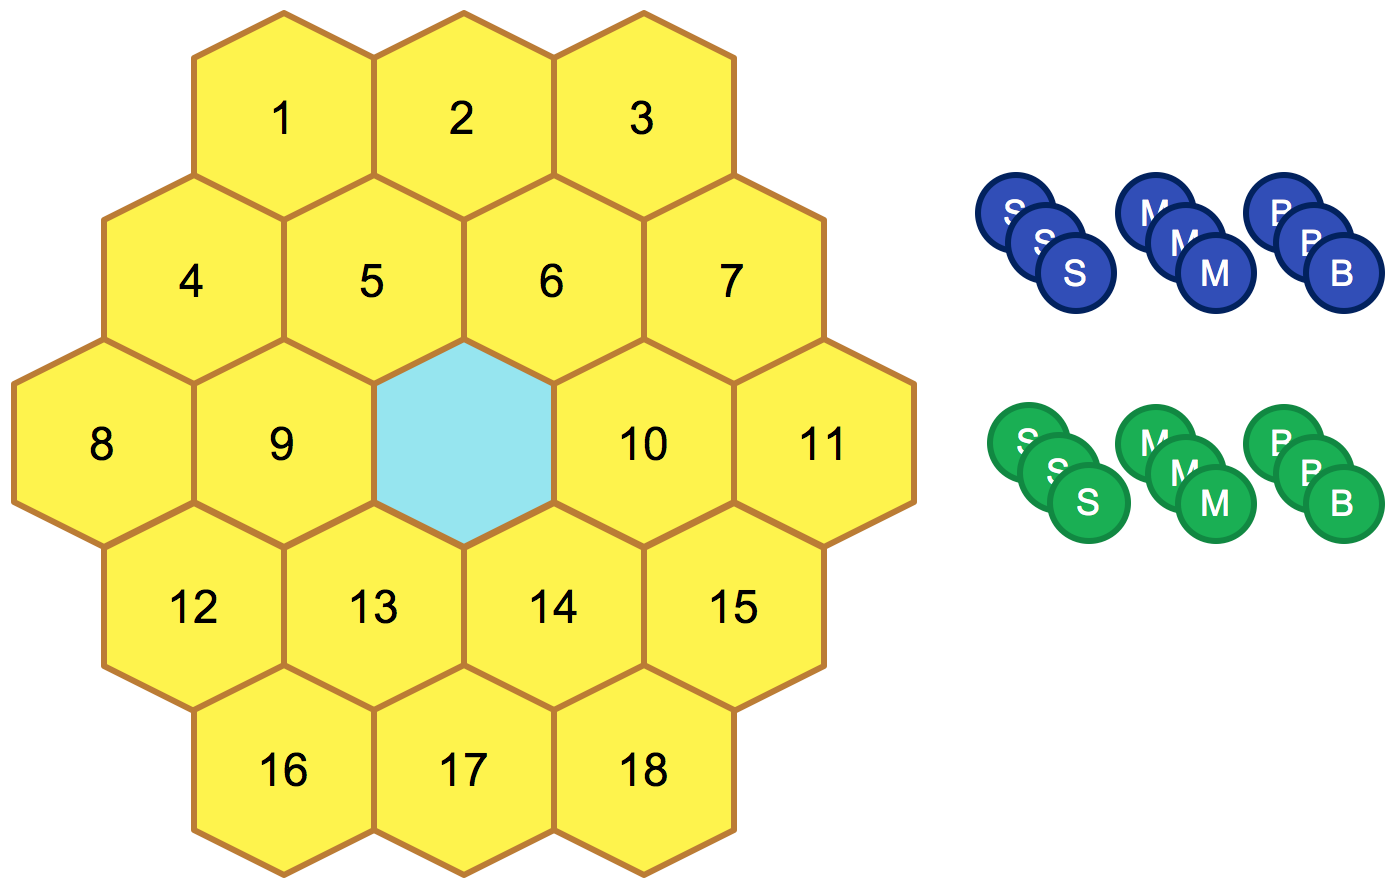
\includegraphics[scale=0.4]{img/board.png}
	\caption{Tabuleiro de jogo}
    \label{Fig:tabuleiro}
	\end{center}
\end{figure}
\newpage
\subsection{Preparação do tabuleiro}

Com um formato hexagonal, o tabuleiro é formado por 18 posições, como é possível observar na figura \ref{Fig:tabuleiro} nas rochas amarelas.
\newline
A cada jogador é atribuído um conjunto de 9 caranguejos: 3 grandes, 3 médios e 3 pequenos, como é possível observar no lado direito da figura \ref{Fig:tabuleiro}.
\newline
Antes do jogo começar, os caranguejos dos jogadores são distribuídos aleatoriamente pelo tabuleiro obedecendo às regras de empilhamento que serão explicitadas na secção \ref{movimentos_caranguejo}.

\subsection{Movimentos possíveis} \label{movimentos_caranguejo}

No turno de um jogador, este pode mover um dos seus caranguejos de forma a terminar o seu movimento numa rocha ocupada por outro caranguejo. Dependendo do seu tamanho, um caranguejo move-se, obrigatoriamente, um determinado número de rochas:
\begin{itemize}
\item Pequeno - move-se três rochas;
\item Médio - move-se duas rochas;
\item Grande - move-se uma rocha.
\end{itemize}
No final do movimento, um caranguejo não pode regressar à rocha inicial.
\newline
Apenas os caranguejos que estejam no topo da pilha podem ser movidos durante o turno de um jogador.
\newline
O empilhamento dos caranguejos tem de obedecer às seguintes regras:
\begin{itemize}
\item um grande pode ficar em cima de qualquer outro caranguejo;
\item um médio pode ficar em cima de um caranguejo médio ou pequeno;
\item um pequeno pode apenas ficar em cima de outro caranguejo pequeno.
\end{itemize}

\subsection{Regra da Onda}
Os caranguejos gostam de estar em grupos grandes e não gostam de ser separados. Numa situação em que os caranguejos fiquem separados em dois grupos, por uma linha de rochas vazias, um destes grupos irá ser eliminado do jogo por uma onda. O grupo a ser eliminado é selecionado pela seguinte ordem de prioridades:
\begin{enumerate}
\item O grupo de caranguejos que ocupar menos espaço no tabuleiro é removido do jogo;
\item Se os dois grupos ocupam o mesmo número de casas no tabuleiro, então o grupo com o menor número total de caranguejos é removido do jogo;
\item Se o número de caranguejos for o mesmo, o jogador do turno em que ocorreu a separação, decide qual o grupo que irá ser removido do jogo.
\end{enumerate}

\subsection{Fim do jogo}

O \textit{Crab Stack} pode terminar nos seguintes estados do jogo:
\begin{itemize}
\item Se todas as peças de um jogador forem removidas do jogo, através de uma onda, o jogador perde o jogo;
\item Se um jogador, no inicio do seu turno, não conseguir mover nenhum dos seus caranguejos, perde o jogo.
\end{itemize}

%%%%%%%%%%%%%%%%%%%%%%%%%%
\newpage

%%%%%%%%%%%%%%%%%%%%%%%%%%
\section{Lógica do Jogo}

Nesta secção é feita uma descrição do projeto e da implementação da lógica do jogo em Prolog, incluindo a forma de representação do estado do tabuleiro e sua visualização, execução de movimentos, verificação do cumprimento das regras do jogo, determinação do final do jogo e cálculo das jogadas a realizar pelo computador utilizando diversos níveis de dificuldade de jogo. 

\subsection{Representação do Estado do Jogo}

\subsubsection{Representação do estado do tabuleiro}

O tabuleiro é representado por uma lista de listas, em que cada elemento da lista representa uma rocha. Os caranguejos de cada jogador serão representados por Sx, Mx, Bx, em que x representa o número do jogador e S, M, B o tamanho do caranguejo, respetivamente pequeno, médio e grande. Uma rocha, i.e. uma célula da lista, tem dois estados diferentes possíveis: estar vazia ou ter uma pilha de caranguejos. Uma pilha de caranguejos, pode ser por exemplo [B1, S1, S2], em que o elemento B1 representa o topo da pilha.
\\O código para a criação de um tabuleiro é dado por:

\begin{lstlisting}[language=Prolog]
% Initializes Board
init_board(Board):-
        Empty_Board = [ [[],[],[]],
                [[],[],[],[]],
                [[],[],[],[]],
                [[],[],[],[]],
                [[],[],[]]
         ],
        crabs(CrabsList),
        add_crab_init_board(Empty_Board, CrabsList, Board).

% Adds the crabs to empty board cells 
add_crab_init_board(Board, [], Board).

add_crab_init_board(Board, [HCrabs | TCrabs], FinalBoard):-
        aux_board(Board, HCrabs, Tmp_FinalBoard),
        add_crab_init_board(Tmp_FinalBoard, TCrabs, FinalBoard),!.

% Auxiliary function to put a crab in an empty cell with random
aux_board(Board, Crab, FinalBoard):-
        repeat,
        random(1, 19, Rock),
        \+ (get_rock(Rock, Board, _)),
        add_crab_board(Board, Rock, Crab, FinalBoard).

\end{lstlisting}

\subsubsection{Posições iniciais do jogo}

No início do jogo, as peças de cada jogador são colocadas aleatoriamente no tabuleiro, garantindo que fica com todas as rochas ocupadas. Abaixo segue-se o predicado que inicia o jogo e um exemplo de um tabuleiro no estado inicial do jogo.
\begin{lstlisting}[language=Prolog]
Board =  [ %initial board example
    	 	[['S1'],['M2'],['M1']],
         	[['B2'],['B1'],['M1'],['S2']],
         	[['S2'],['S1'],['M2'],['B2']],
    	 	[['M2'],['B2'],['S1'],['B1']],
    	 	[['M1'],['S2'],['B1']]]   
\end{lstlisting}

Para uma melhor visualização do estado inicial representado acima, segue-se uma figura ilustrativa.

\begin{figure}[!ht]
	\begin{center}
	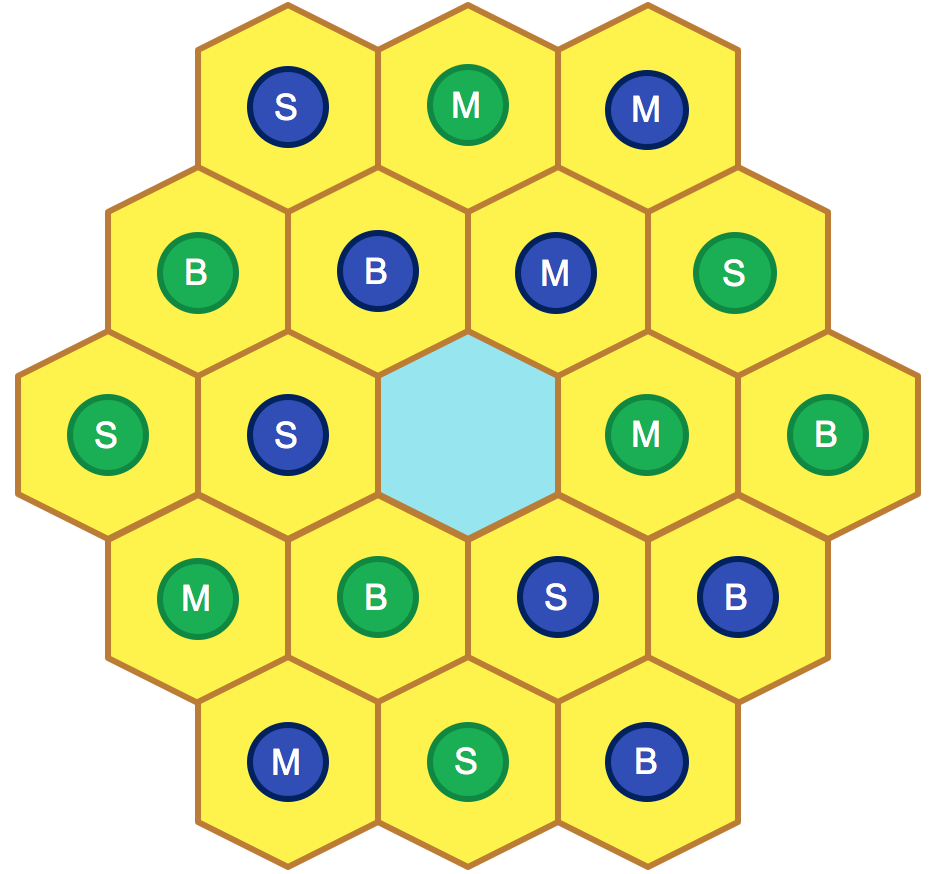
\includegraphics[scale=0.29]{img/init_board.png}
	\caption{Estado inicial do jogo}
    \label{Fig:tabuleiro_inicial}
	\end{center}
\end{figure}

\newpage

\subsubsection{Posições intermédias do jogo} \label{section:intermedia}

Abaixo seguem-se exemplos de tabuleiros num estado intermédio do jogo.

\begin{lstlisting}[language=Prolog]

Board =  [%General Intermediate state board
    	 	[['M1','M2','S1'],[],[]],
         	[[],['B1'],['M1'],['S2']],
         	[['B2','S2'],['S1'],['M2'],['B1','B2']],
    	 	[['B2','M2'],[],['B1','S1'],[]],
    	 	[[],['M1','S2'],[]]]
         
Board =  [% Intermediate state board With a possibility for a wave
    	 	[[],['S1'],['M1']],
         	[['B2'],['M1'],['B1'],['S2']],
         	[[],['S2'],['B1','M2'],['B1','B2']],
    	 	[['M1','M2'],['S1'],[],['S2','S1']],
    	 	[['B2'],['M2'],[]]]
         
Board =  [% Intermediate state board ready for the Wave
    	 	[[],['M1','S1'],['M1']],
         	[['B2'],[],['B1'],['S2']],
         	[[],['S2'],['B1','M2'],['B1','B2']],
    	 	[['M1','M2'],['S1'],[],['S2','S1']],
    	 	[['B2'],['M2'],[]]]
         
Board =  [% Intermediate state board after the Wave
    	 	[[],['M1','S1'],['M1']],
         	[[],[],['B1'],['S2']],
         	[[],[],['B1','M2'],['B1','B2']],
    	 	[[],[],[],['S2','S1']],
    	 	[[],[],[]]]
\end{lstlisting}

Para uma melhor visualização da regra da onda, seguem-se imagens ilustrativas do exemplo apresentado acima, com os diferentes estados intermédios.

\begin{figure}
\begin{tabular}{cc}
  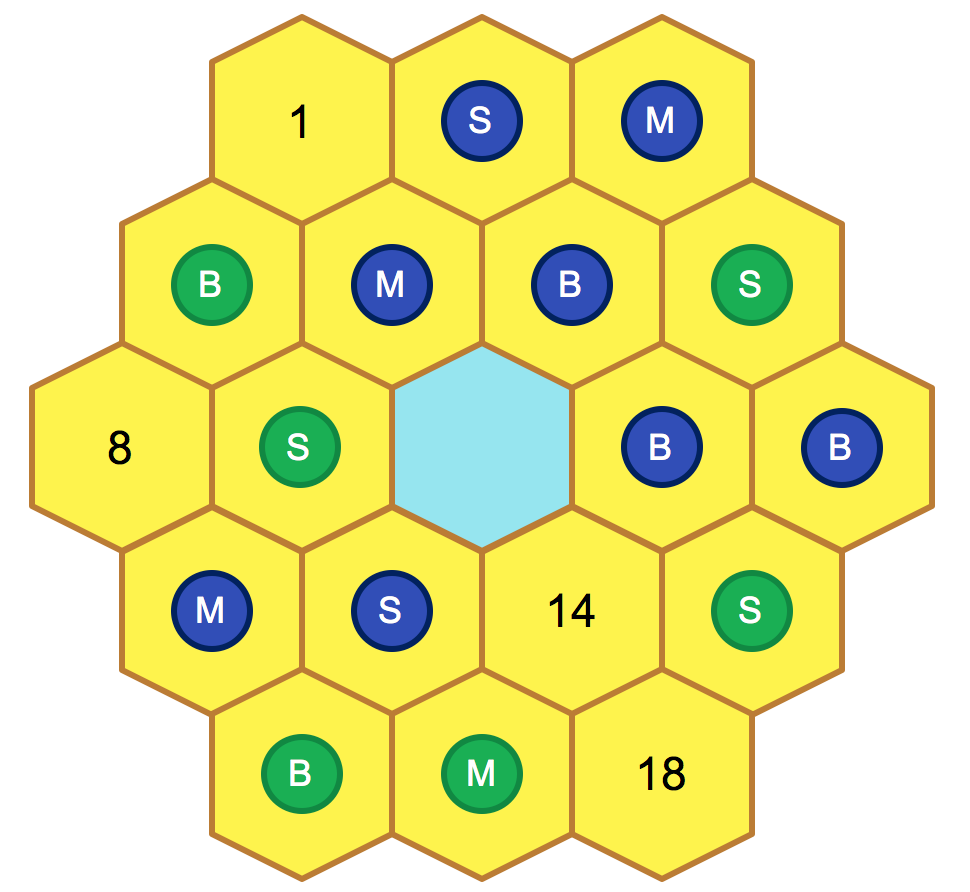
\includegraphics[width=55mm]{img/wave1.png} &   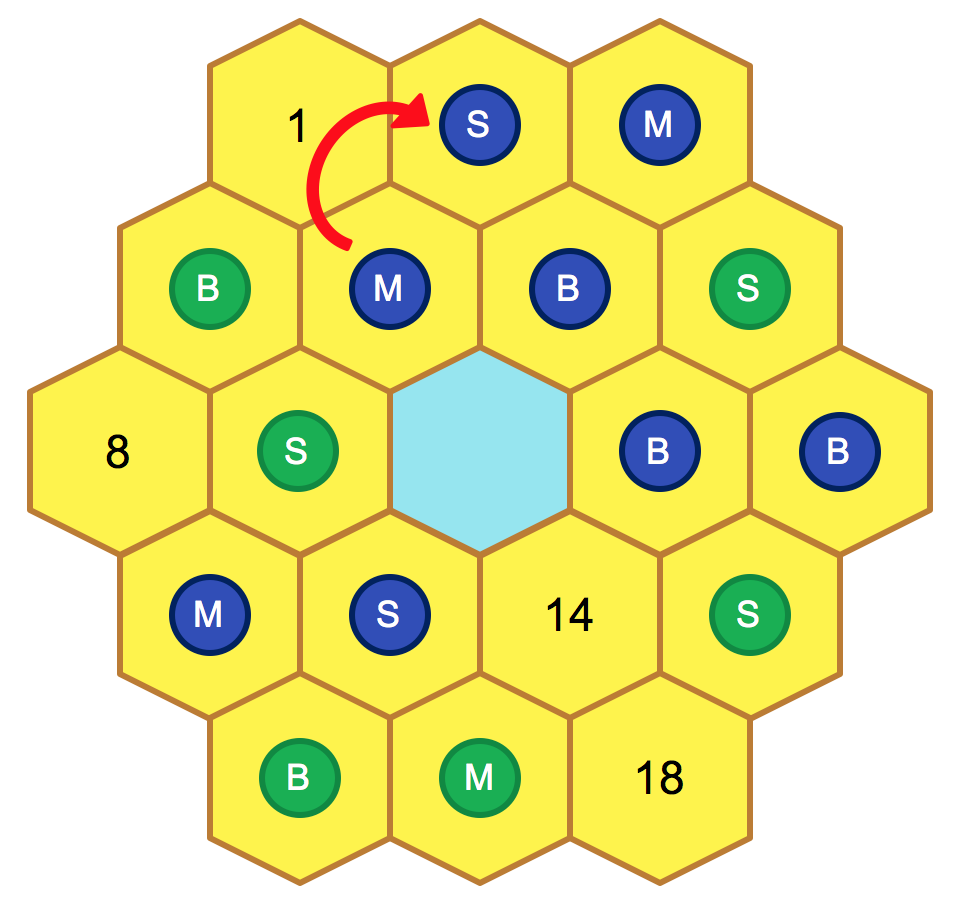
\includegraphics[width=55mm]{img/wave2.png} \\
(a) Possibilidade de ocorrer uma onda. & (b) Jogador azul move peça para  ocorrer uma onda. \\[6pt]
 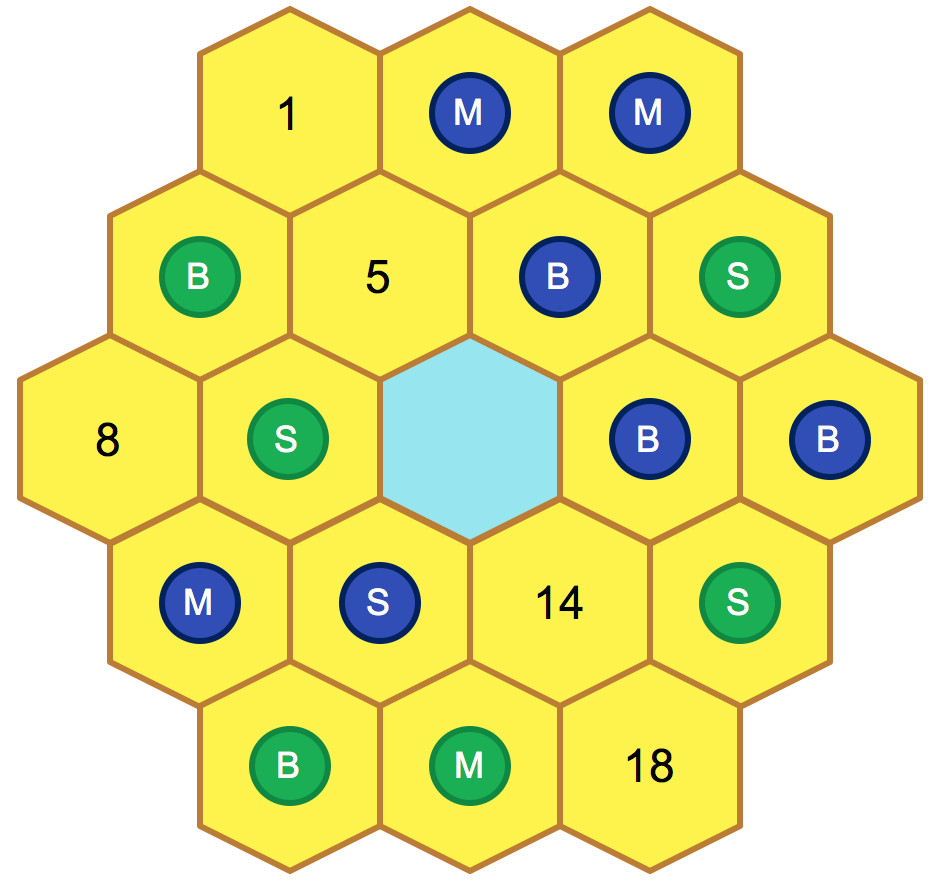
\includegraphics[width=55mm]{img/wave3.png} &   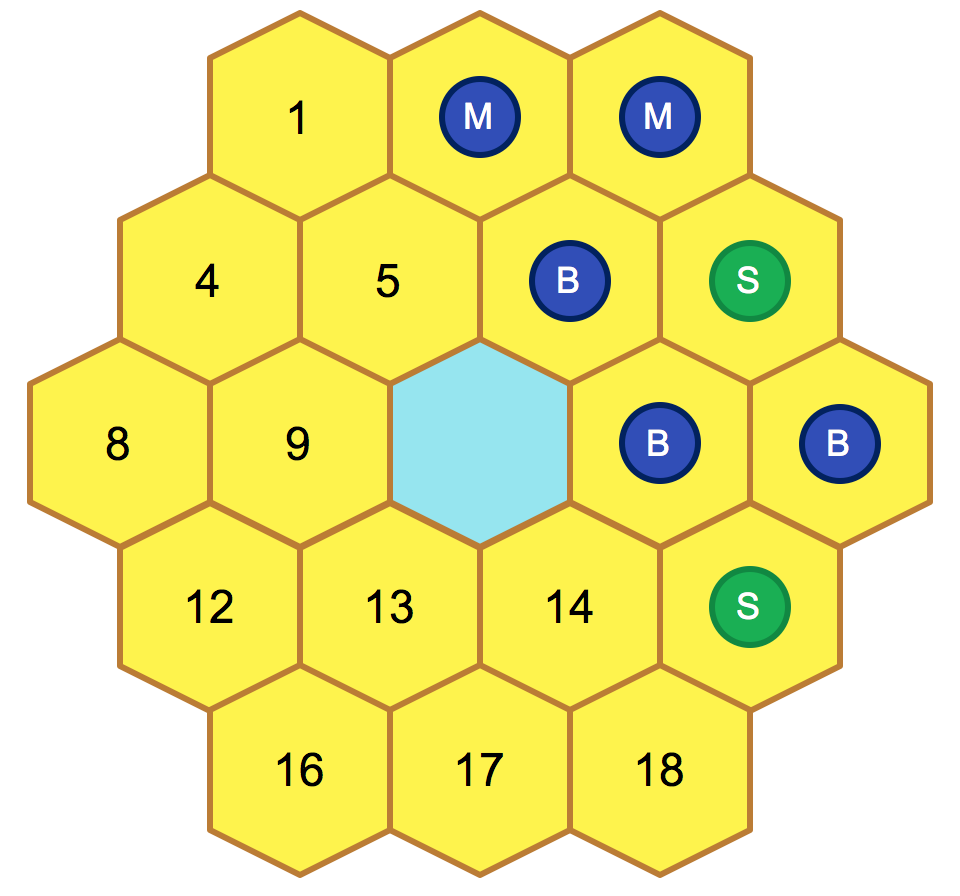
\includegraphics[width=55mm]{img/wave4.png} \\
(c) Ocorre uma onda. & (d) Peças do grupo esquerdo são removidas do jogo. \\[6pt]
\multicolumn{2}{c}{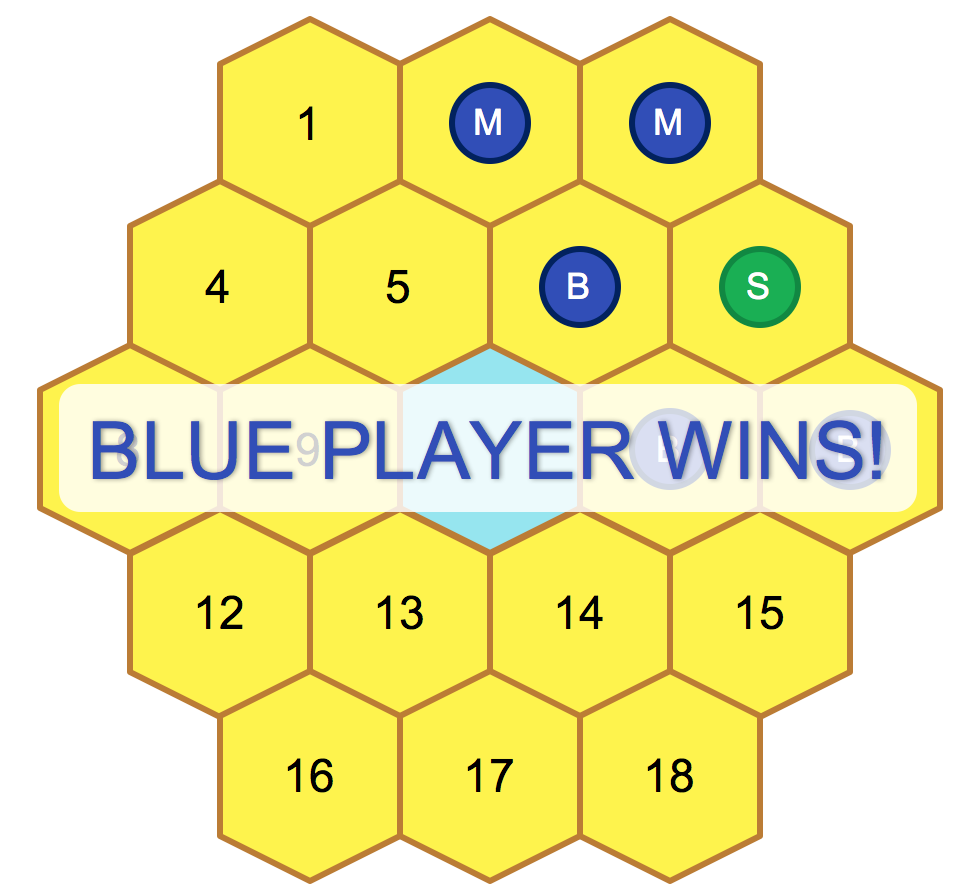
\includegraphics[width=55mm]{img/end_game.png} }\\
\multicolumn{2}{c}{(e) O jogador azul ganha o jogo.}
\end{tabular}
\caption{Exemplo da ocorrência de uma onda durante o turno do jogador azul.}
\label{fig:intermedia}
\end{figure}

\newpage

\subsubsection{Posições finais do jogo}

No exemplo da onda, mencionada na secção anterior, verifica-se que após a onda, o jogador verde apenas pode mover um dos seus caranguejos pequenos para cima do seu outro caranguejo pequeno, deixando de ter movimentos possíveis, e portanto o jogador azul ganha o jogo.
\begin{lstlisting}[language=Prolog]

Board =  [% Green's turn after the wave
    	 	[[],['M1','S1'],['M1']],
         	[[],[],['B1'],['S2']],
         	[[],[],['B1','M2'],['B1','B2']],
    	 	[[],[],[],['S2','S1']],
    	 	[[],[],[]]]
         
Board =  [% Final state board after the green's move
    	 	[[],['M1','S1'],['M1']],
         	[[],[],['B1'],['S2','S2']],
         	[[],[],['B1','M2'],['B1','B2']],
    	 	[[],[],[],['S1']],
    	 	[[],[],[]]]
\end{lstlisting}

%%%%%%%%%%%%%%%%%%%%%%%%%%
\subsection{Visualização do Tabuleiro} 

Para a visualização do tabuleiro, irão ser implementados os seguintes predicados:
\begin{itemize}
\item Cabeçalho do predicado para a visualização do tabuleiro:
\begin{lstlisting}[language=Prolog]
display_board(+Board).
\end{lstlisting}
\item Cabeçalho do predicado para a visualização da pilha:
\begin{lstlisting}[language=Prolog]
display_stack(+Rock, +Stack).
\end{lstlisting}
\end{itemize}

Segue-se a visualização do output do predicado \textit{display\textunderscore board} para o primeiro exemplo de um estado intermédio de jogo apresentado na secção \ref{section:intermedia}.

\begin{figure}[!ht]
	\begin{center}
	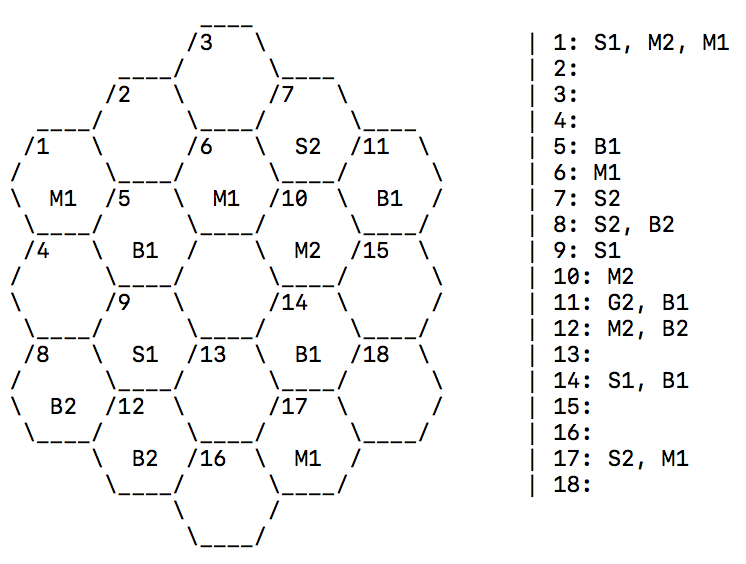
\includegraphics[scale=0.4]{img/display_board.png}
	\caption{Representação do output no estado intermédio do jogo.}
    \label{Fig:display_board}
	\end{center}
\end{figure}

%%%%%%%%%%%%%%%%%%%%%%%%%%
\newpage

\subsection{Lista de Jogadas Válidas}
Para a obtenção de uma lista de jogadas possíveis implementou-se o seguinte predicado \texttt{check\_moves(+Board, +Init\_Pos, +Init\_Crab\_Size, +Final\_Pos, +Player\_Color, +Moves, +ListMoves, -Moves\_Rock, -List\_Moves\_Rock)} que, de forma recursiva, determina se os movimentos são válidos para um dado jogador e para uma dada posição inicial e posição final do tabuleiro. No final, é obtida uma listagem com os movimentos possíveis para uma mesma posição inicial, por exemplo, List\_Moves\_Rock = [[1,2], [1,4]], ou seja, a partir da posição 1 é possível mover um caranguejo para as posições 2 ou 4. O predicado \texttt{moves\_left(+Board, +Player\_Color, +Moves, +List\_Moves\_Counter, +Count, -Final\_Moves, -List\_Final\_Moves)}, chama o \texttt{check\_moves} para as várias posições iniciais e cria uma lista com todas as jogadas possíveis em \texttt{List\_Final\_Moves}.

\subsection{Execução de Jogadas}

O predicado \texttt{make\_move(+Board, +Player, +Player\_Color, -FinalBoard)}, permite ao jogador realizar um movimento. Este predicado faz uma chamada a \texttt{choose\_tile(+Board, +Player, +Player\_Color, -FinalBoard)}, que dependendo se o \texttt{Player} for \textit{human} ou \textit{computer}, questiona ao jogador a posição do caranguejo a mover e a sua posição final, ou determina as posições inicial e final com base na inteligência artificial implementada, respetivamente. 

Os predicados seguintes, foram implementados para validar a jogada introduzida por um jogador \textit{human}. O predicado \texttt{legalMove(+Board, +Rock\_Init, +Rock, +Player\_Color, -FinalBoard)} faz as verificações gerais sobre a legalidade do movimento, tal como, se as posições introduzidas estão dentro do intervalo de rochas do tabuleiro (numeradas de 1 a 18), se existe um caranguejo nessa rocha e se este pertence ao jogador. Para a validação das regras de jogo, é invocado o predicado \texttt{valid\_crab\_movement(+Board, +Rock\_Init, +Rock, +Crab, +Crab\_Size, -FinalBoard)}. Este predicado verifica se a deslocação do caranguejo é válida de acordo com as regras de movimento de um caranguejo dependendo do seu tamanho e se na posição final existe outra caranguejo, dado que estes não se podem deslocar para rochas vazias. Finalmente, se a jogada passar por todos os testes de validação é chamado o predicado \texttt{update\_board(+Board, +Rock, +Rock\_Init, +Crab, -FinalBoard)} que faz a atualização do tabuleiro.


\subsection{Avaliação do Tabuleiro}

O predicado \texttt{evaluate\_board(+Board, +Player, -Value)} permite avaliar um tabuleiro, para um dado jogador, fazendo uso do algoritmo \textit{alphabeta}.
Para o \textit{computer} escolher a sua jogada, é invocado o predicado \texttt{evaluate\_and\_choose(+Board, +Player, +Moves, +Depth, +Alpha, +Beta, +Record, -BestMove)}, que para uma listagem dos movimentos possíveis para um jogador, determina a melhor jogada, a partir da avaliação feita no \texttt{evaluate\_board}. Para avaliar um estado de jogo, fizeram-se as seguintes considerações:
\begin{itemize}
\item Por cada movimento possível, atribui-se um ponto;
\item Por cada caranguejo \textit{Big} do jogador no topo de uma pilha, atribui-se 3 pontos;
\item Por cada caranguejo \textit{Medium} do jogador no topo de uma pilha, atribui-se 2 pontos;
\item Finalmente, por cada caranguejo \textit{Small} do jogador no topo de uma pilha, atribui-se 1 pontos.
\end{itemize}


\subsection{Final do Jogo}
A cada jogada é necessário verificar se o jogo terminou. Para o efeito, criou-se o predicado \texttt{game\_over(+Board, +Winner)} que verifica se a condição de final de jogo foi atingida. O jogo termina, se um jogador ficar sem movimentos possíveis. O predicado \texttt{moves\_left(+Board, +Player\_Color, +Moves, +Count, -Final\_Moves)} calcula o número de jogadas restantes no estado atual de jogo e é invocado pelo predicado \texttt{game\_over}. No caso de \texttt{Final\_Moves} for igual a zero para algum dos jogadores, o outro jogador é declarado vencedor.

%%%%%%%%%%%%%%%%%%%%%%%%%%
\subsection{Jogada do Computador}

A jogada de um \textrm{computer} é feita a partir do predicado
move\_computer(+Board, +Computer\_Color, +Depth, -Computer\_FinalBoard), em que a profundidade indica o nível de dificuldade do computador, que equivale à profundidade de pesquisa no algoritmo \textit{alphabeta}. Os predicados que influenciam na escolha do movimento do computador, são os indicados na secção de Avaliação do Tabuleiro e que são invocados a partir do predicado 
\texttt{alpha\_beta(+Board, +Player, +Depth, +Alpha, +Beta, -Move, -Value)}.

%%%%%%%%%%%%%%%%%%%%%%%%%%
\section{Interface com o Utilizador}

O jogo arranca com a chamada do predicado \textit{crabStack}. É apresentado ao jogador o menu principal \ref{Fig:main_menu}, onde este pode escolher se pretende jogar (\textit{1. Play}), sendo encaminhado para o sub-menu de jogo, ler as regras de jogo (\textit{2. How to play}), conhecer os criadores do jogo (\textit{3. About}) ou sair da aplicação (\textit{4. Exit}). Para uma melhor compreensão dos diferentes sub-menus, estes podem ser consultados no anexo \ref{app:interface}.\\

\begin{figure}[!ht]
	\begin{center}
	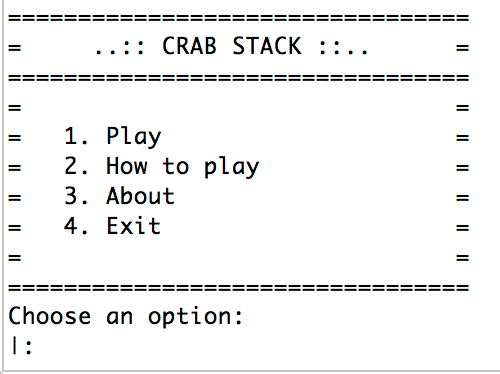
\includegraphics[scale=0.4]{img/main_menu.png}
	\caption{Representação do menu principal.}
    \label{Fig:main_menu}
	\end{center}
\end{figure}

\newpage

Caso o jogador tenha escolhido a opção 1, é encaminhado para o sub-menu de modo de jogo onde pode escolher entre 3 opções de jogo:
\begin{itemize}
\item 1. Jogador vs. Jogador
\item 2. Jogador vs. Computador
\item 3. Computador vs. Computador
\end{itemize}

Se o jogador escolher algum dos modos de computador, terá de introduzir o nível de dificuldade do mesmo.

%%%%%%%%%%%%%%%%%%%%%%%%%%
\section{Conclusões}
Durante este projeto verificou-se um aprofundamento dos conhecimentos em Prolog anteriormente adquiridos durante as aulas e um melhor domínio sobre os mesmos. Este projeto permitiu também, uma melhor compreensão do novo paradigma de programação que a aprendizagem do Prolog exigiu.

O jogo implementado cumpriu as várias regras de jogo descritas e o modo AI foi implementado com sucesso para diferentes níveis de dificuldade, facultados pelo nível de profundidade de pesquisa do algoritmo \textit{alphabeta}. Um aspeto a melhorar, é a eficiência de avaliação e escolha do movimento a efetuar pelo computador.

No geral, concluí-se que o trabalho desenvolvido foi produtivo e positivo, cumprindo todas as especificações exigidas.


\clearpage
\addcontentsline{toc}{section}{Bibliografia}
\renewcommand\refname{Bibliografia}
\bibliographystyle{plain}
\bibliography{myrefs}

\newpage
\appendix
\section{Interface com o utilizador} \label{app:interface}

\subsection{How to play}

\begin{figure}[!ht]
	\begin{center}
	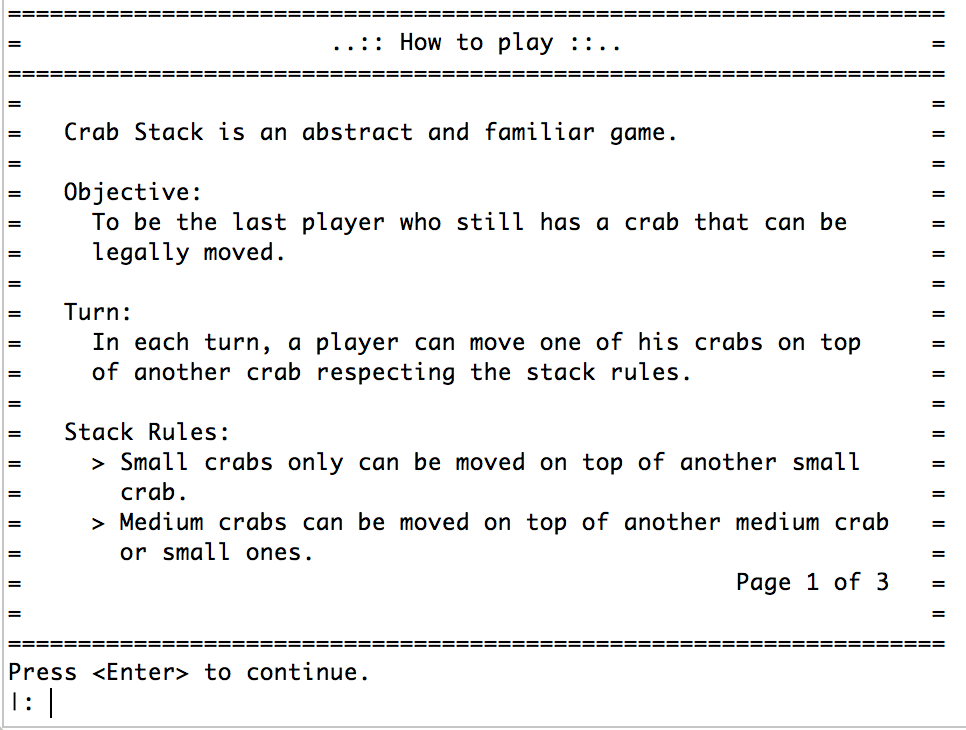
\includegraphics[scale=0.4]{img/how_to_play_1.png}
	\caption{Representação do sub-menu \textit{How to play} página 1.}
    \label{Fig:how_to_play_1}
	\end{center}
\end{figure}

\begin{figure}[!ht]
	\begin{center}
	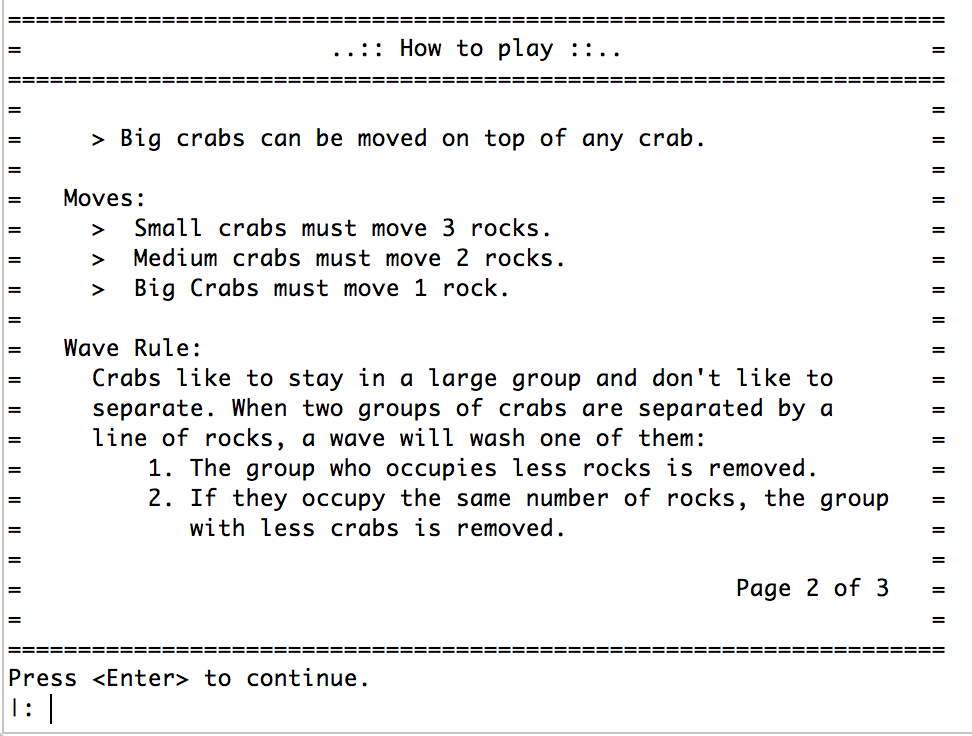
\includegraphics[scale=0.4]{img/how_to_play_2.png}
	\caption{Representação do sub-menu \textit{How to play} página 2.}
    \label{Fig:how_to_play_2}
	\end{center}
\end{figure}

\begin{figure}[!ht]
	\begin{center}
	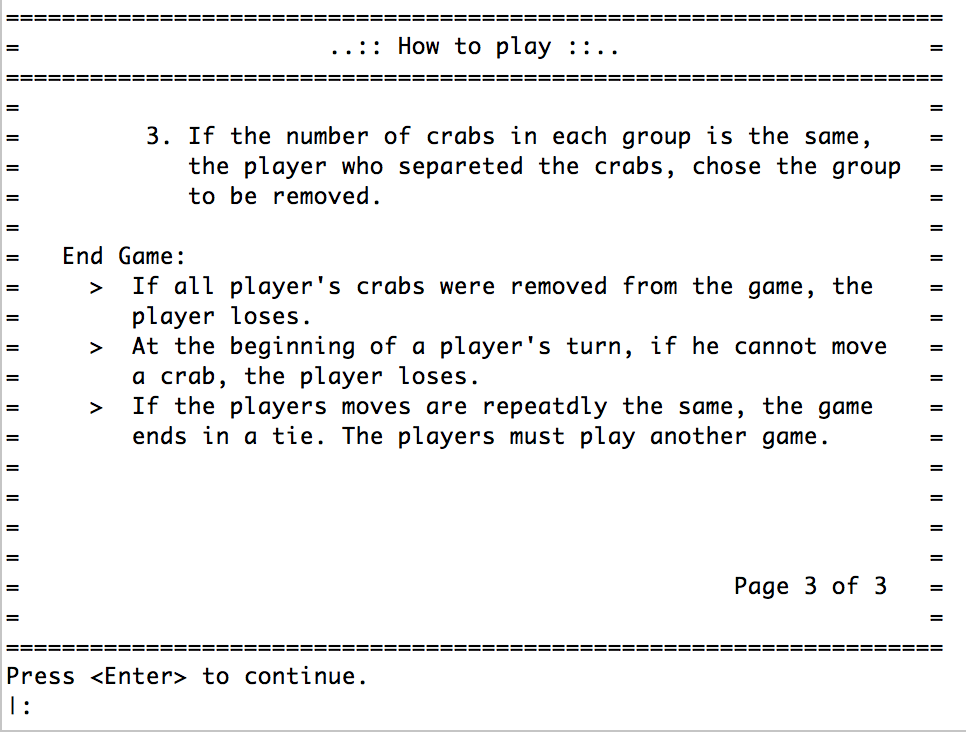
\includegraphics[scale=0.4]{img/how_to_play_3.png}
	\caption{Representação do sub-menu \textit{How to play} página 3.}
    \label{Fig:how_to_play_3}
	\end{center}
\end{figure}

\newpage

\subsection{About}

\begin{figure}[!ht]
	\begin{center}
	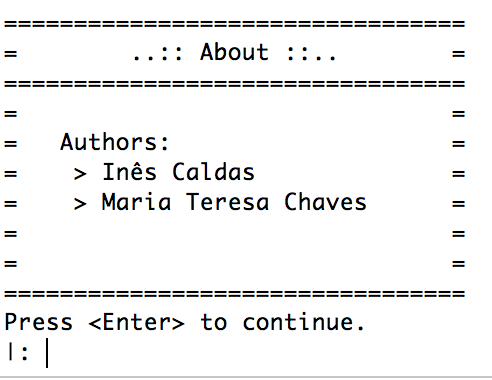
\includegraphics[scale=0.5]{img/about_menu.png}
	\caption{Representação do sub-menu \textit{About}.}
    \label{Fig:about_menu}
	\end{center}
\end{figure}

\subsection{Play}

\begin{figure}[!ht]
	\begin{center}
	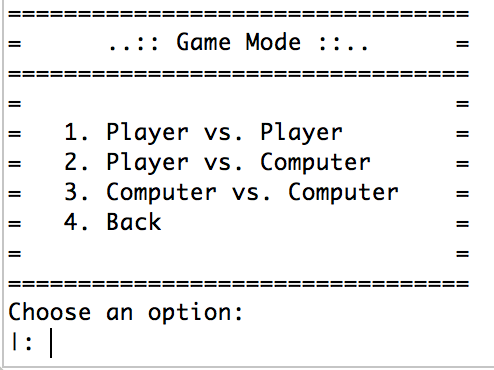
\includegraphics[scale=0.5]{img/play_menu.png}
	\caption{Representação do sub-menu \textit{Play}.}
    \label{Fig:play_menu}
	\end{center}
\end{figure}

\newpage

\subsection{Player vs Player}

\begin{figure}[!ht]
	\begin{center}
	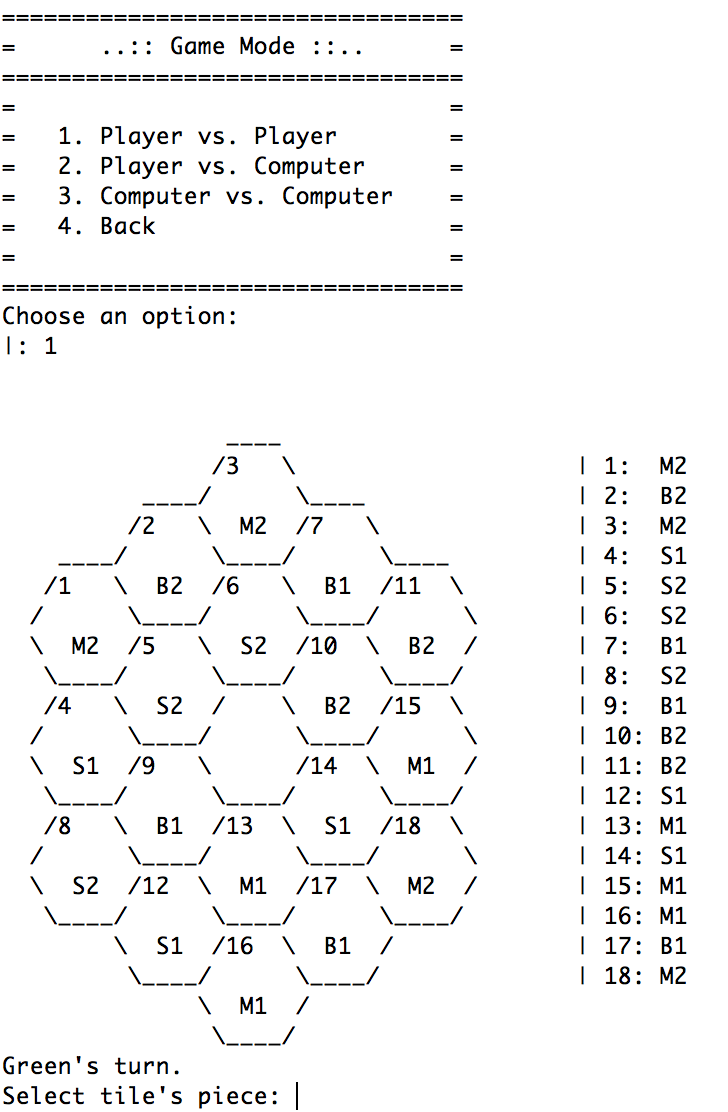
\includegraphics[scale=0.4]{img/player_vs_player.png}
	\caption{Representação do sub-menu \textit{player vs player}.}
    \label{Fig:player_vs_player}
	\end{center}
\end{figure}

\subsection{Player vs Computer}

\begin{figure}[!ht]
	\begin{center}
	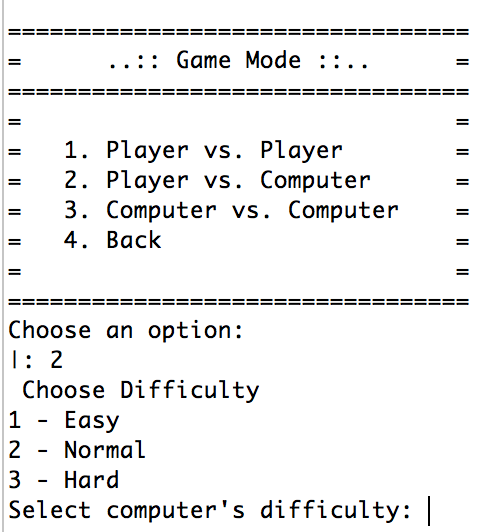
\includegraphics[scale=0.5]{img/player_vs_computer.png}
	\caption{Representação do sub-menu \textit{player vs computer}.}
    \label{Fig:player_vs_computer}
	\end{center}
\end{figure}

\newpage

\subsection{Computer vs Computer}

\begin{figure}[!ht]
	\begin{center}
	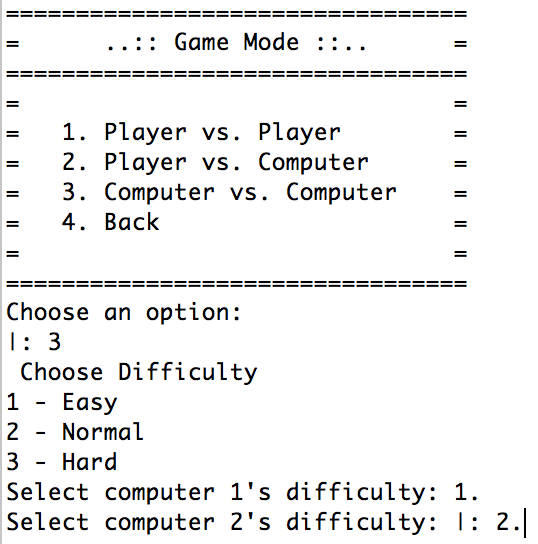
\includegraphics[scale=0.5]{img/computer_vs_computer.png}
	\caption{Representação do sub-menu \textit{computer vs computer}.}
    \label{Fig:computer_vs_computer}
	\end{center}
\end{figure}

\newpage

\section{Código Fonte} \label{app:source_code}

\subsection{crab\_stack.pl}

\begin{mdframed}[linecolor=black, topline=false, bottomline=false,
  leftline=false, rightline=false]
    \inputminted[fontsize=\scriptsize, linenos, breaklines=true]{prolog}{src/crab_stack.pl}
\end{mdframed}

\newpage

\subsection{cs\_ai.pl}

\begin{mdframed}[linecolor=black, topline=false, bottomline=false,
  leftline=false, rightline=false]
    \inputminted[fontsize=\scriptsize, linenos, breaklines=true]{prolog}{src/cs_ai.pl}
\end{mdframed}

\newpage

\subsection{cs\_board.pl}

\begin{mdframed}[linecolor=black, topline=false, bottomline=false,
  leftline=false, rightline=false]
    \inputminted[fontsize=\scriptsize, linenos, breaklines=true]{prolog}{src/cs_board.pl}
\end{mdframed}

\newpage

\subsection{cs\_menus.pl}

\begin{mdframed}[linecolor=black, topline=false, bottomline=false,
  leftline=false, rightline=false]
    \inputminted[fontsize=\scriptsize, linenos, breaklines=true]{prolog}{src/cs_menus.pl}
\end{mdframed}

\newpage

\subsection{cs\_utilities.pl}

\begin{mdframed}[linecolor=black, topline=false, bottomline=false,
  leftline=false, rightline=false]
    \inputminted[fontsize=\scriptsize, linenos, breaklines=true]{prolog}{src/cs_utilities.pl}
\end{mdframed}

\newpage

\end{document}


